\documentclass[11pt,a4paper]{article}

\usepackage[margin=1in]{geometry}
\usepackage[T1]{fontenc}
\usepackage[utf8]{inputenc}
\usepackage{lmodern}
\usepackage{hyperref}
\usepackage{graphicx}
\usepackage{float}
\usepackage{xcolor}
\usepackage{listings}
\usepackage{enumitem}
\usepackage{booktabs}

\hypersetup{
    colorlinks=true,
    linkcolor=blue,
    urlcolor=blue,
    pdftitle={SEDS519 HW1 Report},
    pdfauthor={Student}
}

\lstdefinestyle{pythonstyle}{
    language=Python,
    basicstyle=\ttfamily\small,
    keywordstyle=\color{blue},
    commentstyle=\color{gray},
    stringstyle=\color{teal},
    showstringspaces=false,
    frame=single,
    breaklines=true,
    tabsize=4
}

\title{SEDS519 HW1 Report\\Petition Management System}
\author{Student Name \\ Student ID}
\date{\today}

\begin{document}

\maketitle

\section{Introduction}

This report explains the design and implementation of the Petition Management
System developed for SEDS519 HW1. The application is a desktop GUI program that
allows users to select built-in or user-defined petition templates, create
petitions from scratch, edit petition details, save them as reusable templates,
save them as drafts or register them, and browse saved petitions with filtering
support.

The homework specifically requires the use of the following design patterns:
\begin{itemize}[leftmargin=1.5em]
    \item Factory Method
    \item Singleton
    \item Iterator
    \item Prototype
\end{itemize}

The implementation satisfies these requirements through a petition creation
layer, a central petition registry, a filtered petition iterator, and cloning
support for template-based editing. The final version also includes a separate
template persistence layer so that users can define their own templates from
scratch and reuse them later.

\section{Project Overview}

The system is organized into the following modules:
\begin{itemize}[leftmargin=1.5em]
    \item \texttt{models}: petition domain classes
    \item \texttt{factories}: creation logic for petition subtypes
    \item \texttt{templates}: built-in template catalog
    \item \texttt{registry}: petition and template persistence
    \item \texttt{iterators}: traversal and filtering logic
    \item \texttt{gui}: Flet-based desktop user interface
    \item \texttt{utils}: validation helpers
\end{itemize}

The application starts from \texttt{src/main.py}, launches the Flet GUI, loads
template petitions, loads previously saved petitions from JSON storage, and
allows the user to create editable petition copies from built-in templates,
user-defined templates, or blank petition types.

\section{Factory Method Pattern}

\subsection{Intent}

The Factory Method pattern is used to create petitions of different types
without forcing the client code to directly instantiate concrete petition
classes.

\subsection{Implementation}

The abstract base factory is \texttt{PetitionFactory}. It declares the
\texttt{create\_petition(...)} method and acts as a shared creation interface
for all petition factories.

\begin{lstlisting}[style=pythonstyle,caption={Abstract petition factory}]
class PetitionFactory(ABC):
    @abstractmethod
    def create_petition(
        self,
        title: str,
        body: str,
        petitioner: str,
        created_by: str,
        status: str = "draft",
        attachment_required: bool = False,
        attachments: list[str] | None = None,
    ) -> Petition:
        raise NotImplementedError
\end{lstlisting}

Two concrete factories implement this interface:
\begin{itemize}[leftmargin=1.5em]
    \item \texttt{AcademicPetitionFactory}
    \item \texttt{AdministrativePetitionFactory}
\end{itemize}

Each concrete factory returns a different petition subtype with its own default
receiver and type metadata:
\begin{itemize}[leftmargin=1.5em]
    \item academic petitions default to \texttt{receiver = "Dean"}
    \item administrative petitions default to
    \texttt{receiver = "Administrative Office"}
    \item factory calls can also specify whether attachments are required
\end{itemize}

\subsection{How it is used}

The template catalog uses these factories to create built-in petition templates.
For example, the academic templates are generated by creating an
\texttt{AcademicPetitionFactory} instance and repeatedly calling
\texttt{create\_petition(...)}. The internship approval template is created
with \texttt{attachment\_required=True}, which demonstrates that different
petition instances can carry different rules at creation time.

This design keeps template creation logic centralized and prevents the GUI from
being tightly coupled to concrete petition classes.

\subsection{Why this is appropriate}

Factory Method is appropriate here because the application creates more than one
petition subtype and each subtype may evolve with different defaults, receivers,
or future attachment rules. The pattern makes these differences explicit while
keeping creation logic clean and extensible.

\section{Singleton Pattern}

\subsection{Intent}

The Singleton pattern is used to ensure that the petition registry is shared
across the entire application.

\subsection{Implementation}

The \texttt{PetitionRegistry} class stores a class-level variable named
\texttt{\_instance}. Its \texttt{\_\_new\_\_} method checks whether an instance
already exists:
\begin{itemize}[leftmargin=1.5em]
    \item if not, it creates one object
    \item if yes, it returns the existing object
\end{itemize}

\begin{lstlisting}[style=pythonstyle,caption={Singleton registry creation logic}]
class PetitionRegistry:
    _instance: "PetitionRegistry | None" = None

    def __new__(cls) -> "PetitionRegistry":
        if cls._instance is None:
            cls._instance = super().__new__(cls)
            cls._instance._petitions = []
            cls._instance._storage_dir = (
                Path(__file__).resolve().parents[2] / "data" / "petitions"
            )
            cls._instance._storage_dir.mkdir(parents=True, exist_ok=True)
            cls._instance.load_all_petitions()
        return cls._instance
\end{lstlisting}

\subsection{Responsibilities of the registry}

The registry acts as the single control structure for petitions in the system.
It supports:
\begin{itemize}[leftmargin=1.5em]
    \item adding a petition
    \item registering a petition
    \item retrieving all petitions
    \item retrieving only drafts
    \item retrieving only registered petitions
    \item loading petitions from JSON storage
    \item saving petitions back to JSON storage
\end{itemize}

\subsection{Why this is appropriate}

The homework requires a single shared registry over petitions that are either in
draft state or already registered. Singleton fits this requirement directly
because every part of the application works with the same in-memory petition
collection and the same storage directory. A separate \texttt{TemplateRegistry}
is used for user-defined reusable templates, but the Singleton requirement is
specifically fulfilled by \texttt{PetitionRegistry}.

\section{Iterator Pattern}

\subsection{Intent}

The Iterator pattern is used to traverse petitions stored in the registry while
optionally filtering them by type or status.

\subsection{Implementation}

The \texttt{PetitionIterator} class accepts:
\begin{itemize}[leftmargin=1.5em]
    \item a petition list
    \item an optional petition type filter
    \item an optional status filter
\end{itemize}

It implements both \texttt{\_\_iter\_\_} and \texttt{\_\_next\_\_}, so it can
be used in normal Python iteration constructs.

\begin{lstlisting}[style=pythonstyle,caption={Filtered petition iterator}]
class PetitionIterator:
    def __iter__(self) -> "PetitionIterator":
        return self

    def __next__(self) -> Petition:
        while self._index < len(self._petitions):
            petition = self._petitions[self._index]
            self._index += 1
            matches_type = self._petition_type is None or getattr(
                petition, "petition_type", None
            ) == self._petition_type
            matches_status = self._status is None or petition.status == self._status
            if matches_type and matches_status:
                return petition
        raise StopIteration
\end{lstlisting}

\subsection{How it is used}

The GUI uses \texttt{PetitionIterator} when displaying saved petitions. Instead
of placing filtering logic directly inside the UI, the iterator handles
type-agnostic traversal and optional filtering such as:
\begin{itemize}[leftmargin=1.5em]
    \item academic petitions only
    \item administrative petitions only
    \item draft petitions only
    \item registered petitions only
\end{itemize}

\subsection{Why this is appropriate}

This matches the homework requirement closely: the registry stores the petitions
and the iterator is responsible for traversing them while supporting filtered
views.

\section{Prototype Pattern}

\subsection{Intent}

The Prototype pattern is used to create a new editable petition by copying an
existing petition template.

\subsection{Implementation}

The base \texttt{Petition} model defines a \texttt{clone()} method that returns
a deep copy:

\begin{lstlisting}[style=pythonstyle,caption={Prototype cloning support}]
@dataclass
class Petition:
    ...
    def clone(self) -> "Petition":
        return deepcopy(self)
\end{lstlisting}

\subsection{How it is used}

The built-in petition templates are created once through the factory layer.
User-defined templates are stored separately and loaded from template storage.
When the user selects any template in the GUI, the selected template is cloned
and the clone becomes the editable petition instance. This ensures that:
\begin{itemize}[leftmargin=1.5em]
    \item the original template remains unchanged
    \item every user works on a separate petition object
    \item copying works for both academic and administrative petition types
    \item the same template can be reused many times
\end{itemize}

\subsection{Why this is appropriate}

Prototype is well-suited to template-based petition creation. The user starts
from an existing petition shape, copies it, and customizes the copy instead of
constructing a new object from zero.

\section{Validation Logic}

The homework asks for validity checking, especially for empty petition bodies
and missing attachments when attachments are required.

This logic is implemented in \texttt{utils/validators.py}:

\begin{lstlisting}[style=pythonstyle,caption={Petition validity rules}]
def is_valid_petition(petition: Petition) -> bool:
    if not petition.body.strip():
        return False
    if petition.attachment_required and not petition.attachments:
        return False
    return True
\end{lstlisting}

This helper is used by the GUI before a petition is saved or registered. As a
result, invalid petitions are rejected before they enter persistent storage. In
the final version, the \texttt{Internship Approval Request} template is
configured to require attachments, so the validation rule is now demonstrated by
an actual petition flow rather than only existing as a helper.

\section{GUI Design}

The application includes a desktop GUI built with the Flet framework. The GUI
supports the main user tasks required by the assignment:
\begin{itemize}[leftmargin=1.5em]
    \item browsing built-in petition templates
    \item browsing user-defined templates
    \item creating a blank academic or administrative petition from scratch
    \item selecting a template for editing
    \item editing title, body, petitioner, receiver, and creator fields
    \item saving the current editor state as a reusable template
    \item attaching files
    \item saving a petition as draft
    \item registering a petition
    \item browsing already saved petitions
    \item filtering saved petitions by type and status
\end{itemize}

The GUI is event-driven. Button clicks and dropdown changes trigger handler
functions that delegate work to the registry, validation helper, and iterator.
This keeps the interface responsive while separating display logic from core
petition logic.

\section{Persistence}

Petitions are persisted as JSON files under \texttt{data/petitions}. The
registry is responsible for all persistence:
\begin{itemize}[leftmargin=1.5em]
    \item \texttt{save\_all\_petitions()} serializes petitions to JSON
    \item \texttt{load\_all\_petitions()} reconstructs petition objects on startup
\end{itemize}

The registry also restores the correct petition subtype from stored data. If
\texttt{petition\_type} is academic, it rebuilds an \texttt{AcademicPetition};
if it is administrative, it rebuilds an
\texttt{AdministrativePetition}. Otherwise, it falls back to the base
\texttt{Petition} class.

Reusable user-defined templates are persisted separately under
\texttt{data/templates}. This logic is handled by \texttt{TemplateRegistry},
which mirrors the save/load responsibilities of the petition registry without
being part of the Singleton requirement.

\section{UML Class Diagram}

The project includes a UML class diagram source in the \texttt{docs/uml} folder.
The source was updated to reflect:
\begin{itemize}[leftmargin=1.5em]
    \item the new \texttt{TemplateRegistry}
    \item the revised factory method signature with
    \texttt{attachment\_required}
    \item the GUI support for starting petitions from scratch and saving custom
    templates
\end{itemize}

Figure~\ref{fig:uml} presents the class diagram used to describe the class
structure and interactions.

\begin{figure}[H]
    \centering
    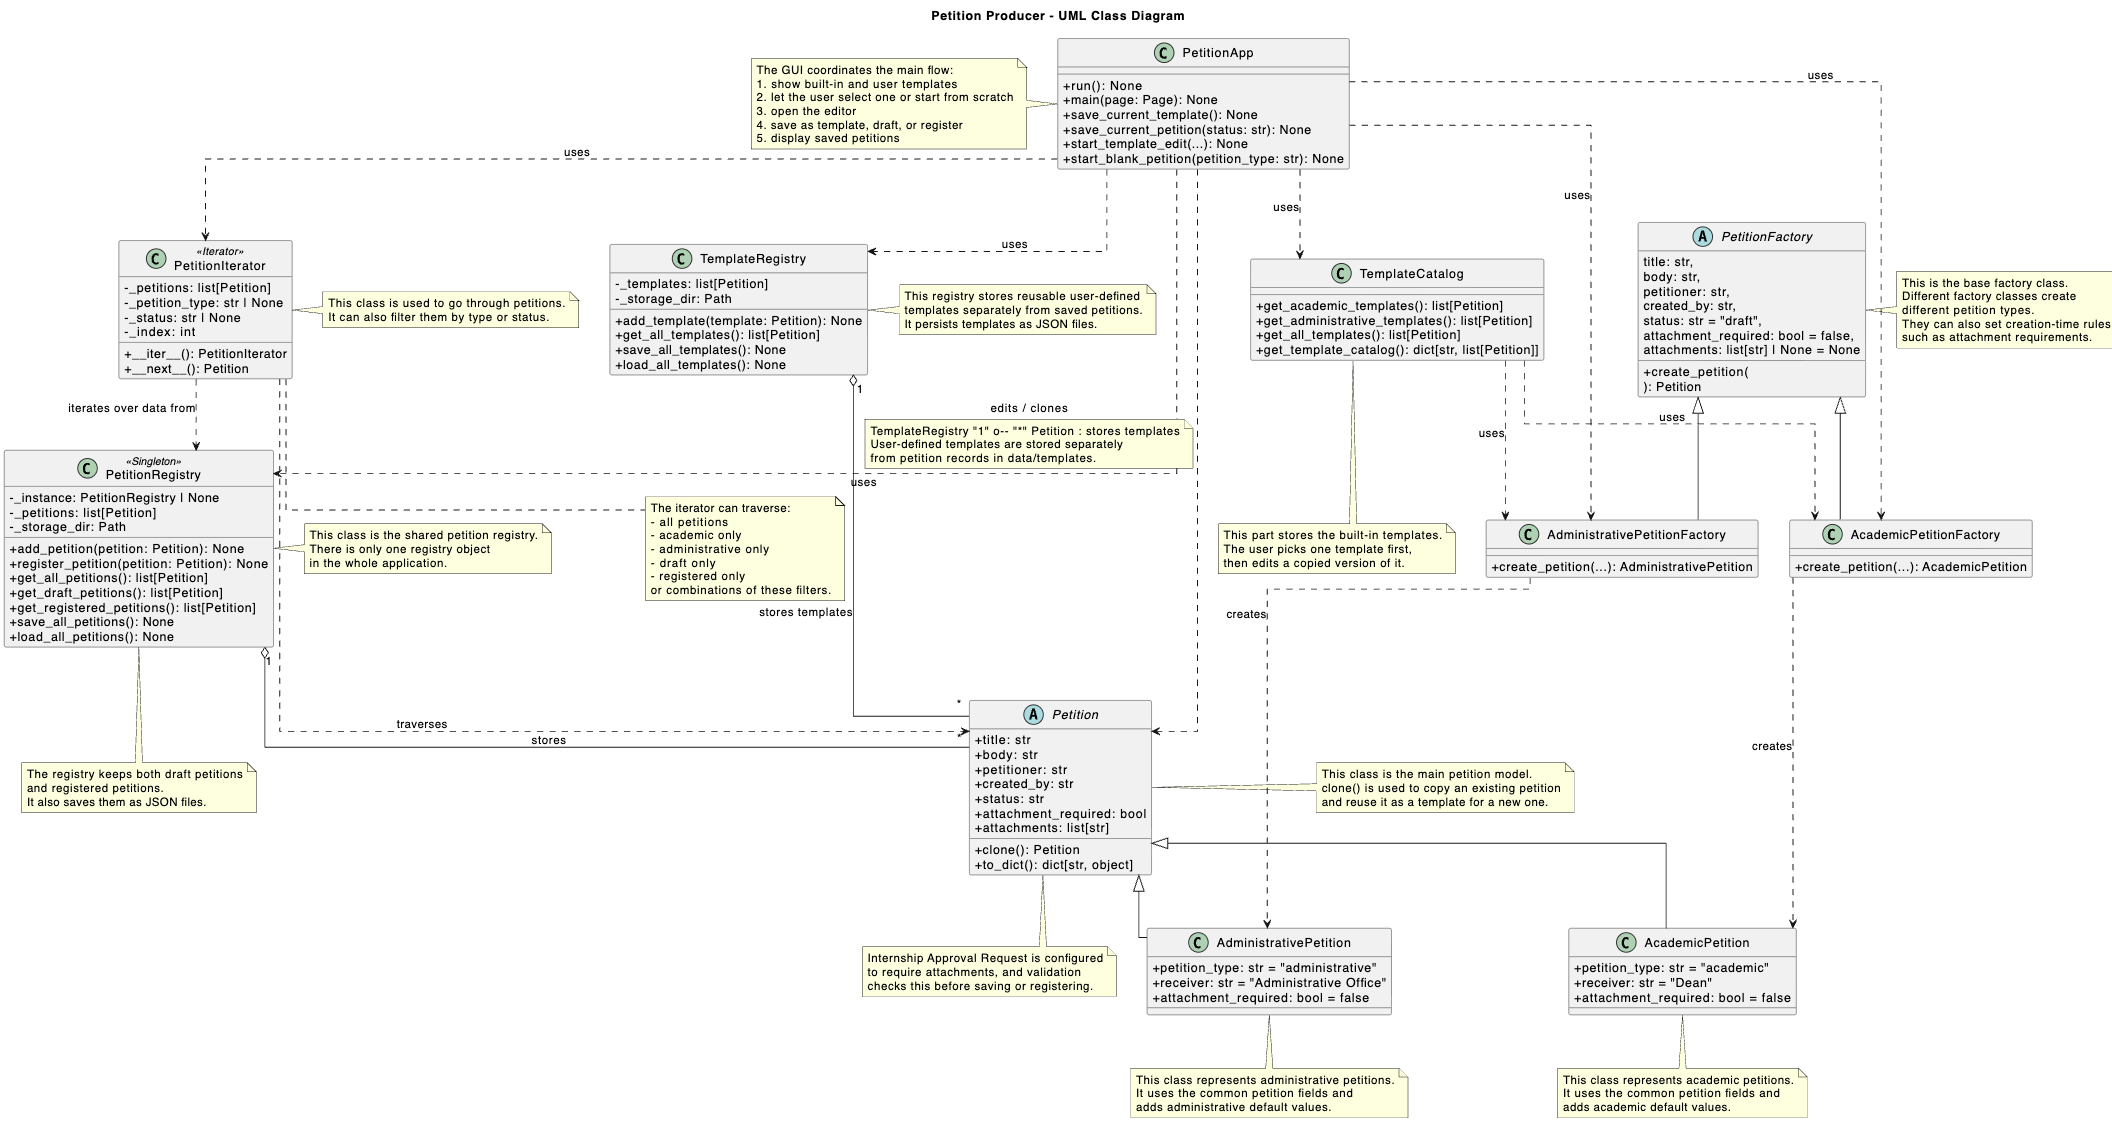
\includegraphics[width=\textwidth]{uml/class_diagram.png}
    \caption{UML class diagram of the Petition Management System}
    \label{fig:uml}
\end{figure}

\section{Requirement Coverage}

\begin{table}[H]
    \centering
    \begin{tabular}{p{0.28\textwidth} p{0.62\textwidth}}
        \toprule
        Requirement & Implementation Summary \\
        \midrule
        Factory Method & Implemented via \texttt{PetitionFactory},
        \texttt{AcademicPetitionFactory}, and
        \texttt{AdministrativePetitionFactory}; also used to configure
        attachment requirements during petition creation. \\
        Singleton & Implemented via \texttt{PetitionRegistry} and its
        class-level \texttt{\_instance}. \\
        Iterator & Implemented via \texttt{PetitionIterator} with optional
        type and status filtering. \\
        Prototype & Implemented via \texttt{Petition.clone()} using
        deep copy. \\
        Validation & Implemented in
        \texttt{utils/validators.py}, including the internship template's
        attachment requirement. \\
        GUI & Implemented with Flet in the \texttt{gui} package, including
        built-in templates, custom templates, and blank petition creation. \\
        UML & Included in \texttt{docs/uml}. \\
        \bottomrule
    \end{tabular}
    \caption{Homework requirement coverage}
\end{table}

\section{Conclusion}

The Petition Management System demonstrates the required design patterns in a
coherent application rather than as isolated examples. Factory Method is used to
create different petition subtypes, Singleton centralizes petition storage,
Iterator provides filtered traversal over saved petitions, and Prototype enables
template cloning for new petition creation. The system also includes validation,
JSON persistence for both petitions and templates, a usable GUI, and UML
documentation.

Overall, the design keeps responsibilities separated and makes the system easier
to extend. New petition types, additional validation rules, or new registry
operations can be added without major restructuring of the current codebase.

\end{document}
